\documentclass[../../main.tex]{subfiles}
\begin{document}
In diesem Kapitel sei stets $K$ ein Körper.

\section{Charakteristisches Polynom und Eigenwerte}

\begin{notrep}\label{10.1.1}
[$\to$ \ref{7.1.6}, \ref{6.3.1}] Ist $V$ ein $K$-Vektorraum, so ist
\begin{align*}
\End(V) := \Hom(V,V) & = \left\{f\mid f\text{ Endomorphismus der Vektorraums }V\right\}\\
& = \left\{f\mid f\colon V\to V \text{ linear}\right\}
\end{align*}
ein Unterraum des $K$-Vektorraums $V^V$\index{Vektorraum@{\bf Vektorraum}!Homomorphismus/ lineare Abbildung!End@$\End(V)$}.
\end{notrep}

\begin{df}\label{10.1.2}
Sei $V$ ein $K$-Vektorraum und $f\in \End(V)$. Es heißt $\lambda\in K$ ein \emph{Eigenwert}\index{Vektorraum@{\bf Vektorraum}!Homomorphismus/ lineare Abbildung!Eigenwert} (\emph{EW}) von $f$, wenn es ein $v\in V$ gibt mit $v\ne 0$ und $f(v) = \lambda v$. Jedes solche $v$ heißt ein \emph{Eigenvektor}\index{Vektorraum@{\bf Vektorraum}!Homomorphismus/ lineare Abbildung!Eigenvektor} (\emph{EV}) von $f$ zum Eigenwert $\lambda$. Für jeden Eigenwert $\lambda$ von $f$ nennt man den Unterraum \[\ker(f-\lambda\id_V) = \left\{v\in V\mid f(v) = \lambda v\right\}\subseteq V,\] welcher aus dem Nullvektor und den Eigenvektoren zum Eigenwert $\lambda$ besteht, den \emph{Eigenraum}\index{Vektorraum@{\bf Vektorraum}!Homomorphismus/ lineare Abbildung!Eigenraum} von $f$ zum Eigenwert $\lambda$.
\end{df}

\begin{bsp}\label{10.1.3}
[$\to$ \ref{6.3.2}, \ref{7.1.4}]
\begin{enumerate}[\normalfont(a)]
\item Die Drehung $R_\ph$ um den Winkel $\ph\in \R$, hat nur dann einen Eigenwert, wenn $\ph = n\pi$ für ein $n\in \Z$. Ist $\ph = n\pi$ für ein \case{gerades}{ungerades} $n\in \Z$, so ist \case{$+1$}{$-1$} der einzige Eigenwert von $\ph$ und jedes $v\in \R^2\setminus\left\{0\right\}$ ein Eigenvektor zu diesem Eigenwert (und damit $\R^2$ der Eigenraum zu diesem Eigenwert).
\item Die Spiegelung $S$ hat die Eigenwerte $1$ und $-1$. Es ist $\lin\cvec{0\\1}$ der Eigenraum zum Eigenwert $1$ und $\lin\cvec{1\\0}$ der Eigenraum zum Eigenwert $-1$.
\item Die Projektion $P$ hat die Eigenwerte $1$ und $0$. Es ist $\lin\cvec{1\\0}$ der Eigenraum zum Eigenwert $1$ und $\lin\cvec{0\\1}$ der Eigenraum zum Eigenwert $0$.
\item Der einzige Eigenwert der Scherung $T_a$ ($a\in \R$) ist $1$. Falls $a = 0$, so ist $\R^2$ der dazugehörige Eigenraum, sonst $\lin\cvec{1\\0}$.
\begin{center}
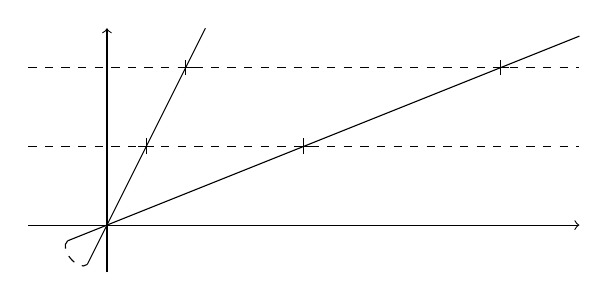
\begin{tikzpicture}
\draw[->] (-1,0) -- (6,0);
\draw[->] (0,-.6) -- (0,2.5);

\draw (.5,.9) -- (.5,1.1);
\draw (.4,1) -- (.6,1);

\draw (1,1.9) -- (1,2.1);
\draw (.9,2) -- (1.1,2);

\draw[dashed] (-1,1) -- (6,1);
\draw[dashed] (-1,2) -- (6,2);

\draw (-.25,-.5) -- (.5,1) -- (1,2) -- (1.25,2.5);

\draw (2.5,.9) -- (2.5,1.1);
\draw (2.4,1) -- (2.6,1);

\draw (5,1.9) -- (5,2.1);
\draw (4.9,2) -- (5.1,2);

\draw (-.5, -.2) -- (2.5,1) -- (5,2) -- (6,2.4);

\path[dashed] (-.5, -.2) edge[bend right = 90] (-.25, -.5);
\end{tikzpicture}
\end{center}
\item Ist $A\in K^{n\times n}$, so ist $f_A : K^n\to K^n, x\mapsto Ax$ ein Endomorphismus von $K^n$. Man spricht dann auch von Eigenwert, Eigenvektor und Eigenräumen \emph{von $A$} statt \emph{von $f_A$}. Es ist also $\lambda\in K$ ein Eigenwert von $A$, wenn es ein $x\in K^n$ gibt mit $x\ne 0$ und $Ax = \lambda x$.
Jedes solche $x$ heißt ein Eigenvektor von $A$ zum Eigenwert $\lambda$. Ist $\lambda$ ein Eigenwert von $A$, so ist $\ker(A-\lambda I_n)\subseteq K^n$ der dazugehörige Eigenraum.
\item Die formale Ableitung $D\colon K[X]\to K[X]$ hat nur den Eigenwert $0$. Es ist zum Beispiel $1$ ein Eigenvektor zu diesem Eigenwert. Für $K = \R$ ist der zugehörige Eigenraum gleich $\R$. Im Allgemeinen ist der Eigenraum komplizierter, denn es ist für $K = \F_2$ auch $X^2$ ein Eigenvektor zum Eigenwert $0$, denn $X^2 \ne 0$ und $D(X^2) = 2X = 0\cdot X = 0$.
\item Die Auswertung $E_{a_1,\ldots,a_n}$ ist zwar eine lineare Abbildung, aber kein Endomorphismus, weswegen die Begriffe Eigenwert und Eigenvektor dafür keinen Sinn machen.
\item Als Endomorphismus des $\R$-Vektorraums $\C$ hat die komplexe Konjugation $C$ die Eigenwerte $1$ und $-1$. Es ist $\R$ der Eigenraum zum Eigenwert $1$ und $\left\{x\i\mid x\in\R\right\}$ der Eigenraum zum Eigenwert $-1$.
\end{enumerate}
\end{bsp}

\begin{lem}\label{10.1.4}
Sei $V$ ein $K$-Vektorraum mit $n:=\dim V<\infty$ und geordneten Basen $\v$ und $\w$. Sei $f\in \End(V)$. Dann sind die beiden Matrizen \[M(f,\v) - XI_n, M(f,\w)- \underbrace{XI_n}_{\llap{$=
\begin{pmatrix}
      X& \multicolumn{2}{c}{\text{\kern 1em\smash{\raisebox{-1.5ex}{\Huge$0$}}}} \\
      & \ddots &  \\
      \multicolumn{2}{c}{\text{\kern-1.5em\smash{\raisebox{0ex}{\Huge$0$}}}} &X
    \end{pmatrix}
$}}\in K[X]^{n\times n}\]
ähnlich {\rm[$\to$ \ref{9.1.16}]} und haben daher dieselbe Determinante {\rm[$\to$ \ref{9.1.18}]}.
\end{lem}
\begin{proof}
Nach \ref{9.1.19} gilt $M(f,\v)\approx M(f,\w)$, das heißt es gibt ein invertierbares $P\in K^{n\times n}$ mit $M(f,\v) = P^{-1}M(f,\w)P$. Es folgt
\begin{align*}
P^{-1}(M(f,\w)- XI_n)P &= P^{-1}M(f,\w)P - P^{-1}(XI_n)P\\
&\overset{\ref{7.2.7}(b)}= M(f,\v) - XP^{-1}P = M(f,\v) - XI_n
\end{align*}
und daher $M(f,\v) - XI_n \approx M(f,\w) - X I_n$.
\end{proof}

\begin{df}\label{10.1.5}
Sei $V$ ein endlichdimensionaler Vektorraum und $f\in \End(V)$. Dann ist das \emph{charakteristische Polynom}\index{Vektorraum@{\bf Vektorraum}!charakteristisches Polynom} von $f$ definiert als \[\chi_f := \det(M(f,\v)- XI_n)\in K[X],\] wobei $\v$ eine beliebig gewählte Basis von $V$ ist [$\to$ \ref{10.1.4}].
\end{df}

\begin{bem}\label{10.1.6}
Sei $V$ ein $K$-Vektorraum, $n:= \dim V < \infty$ und $f\in \End(V)$. Dann gibt es $a_0,\ldots,a_{n-1}\in K$ mit $\chi_f = (-1)^nX^n+ a_{n-1}X^{n-1} + \ldots + a_1X_1+a_0$, wobei $a_0 = \det f$. Insbesondere hat $\chi_f$ den Grad $n$.
Dies folgt leicht aus der Leibniz-Formel \ref{9.1.7}\eqref{leibniz}, weil $M(f,\v)- XI_n)$ von der Form
\[\begin{pmatrix}
b_{11}-X &\multicolumn{2}{c}{\text{"`aus $K$"'}}\\
& \ddots\\
\multicolumn{2}{c}{\text{"`aus $K$"'}} & b_{nn}-X
\end{pmatrix}\]
ist.
\end{bem}

\begin{pro}\label{10.1.7}
Sei $V$ ein $K$-Vektorraum, $n:=\dim V < \infty$, $f\in \End(V)$ und $\lambda\in K$. Dann
\[\lambda\text{ Eigenwert von }f \text{ \rm[$\to$ \ref{10.1.2}]} \iff \chi_f(\la) = 0 \text{ \rm[$\to$ \ref{writepx}]}.\]
"`Die Eigenwerte sind die Nullstellen {\rm[$\to$ \ref{4.2.9}]} des charakteristischen Polynoms."'
\end{pro}
\begin{proof} Wähle eine geordnete Basis $\v$ von $V$.
\begin{align*}
\lambda\text{ Eigenwert von } f & \overset{\ref{10.1.2}}{\iff} \exists v\in V\setminus \left\{0\right\}: f(v) = \lambda v\\
& \iff \ker(f-\lambda\id_V)\ne \left\{0\right\}\\
& \overset{\ref{6.2.25} \text{(b)}}{\iff} \dim \ker (f-\lambda\id_V) \ne 0\\
& \overset{\ref{8.1.12}}{\iff} \dim\im (f-\lambda\id_V)\ne n\\
& \overset{\ref{8.1.15}}{\iff} \rank (M(f-\lambda\id_V,\v))\ne n\\
& \overset{\ref{8.1.16}}{\iff} M(f- \lambda\id_V,\v) \text{ nicht invertierbar}\\
& \overset{\ref{9.1.14}}{\iff} \det\underbrace{M(f-\lambda\id_V,\v)}_{\overset{\ref{7.1.8}}{=} M(f,\v) - \lambda \underbrace{\scriptstyle M(\id_V,\v)}_{\overset{\ref{7.2.10}}{=} I_n}} = 0\\
&\iff \det(M(f,\v)-\lambda I_n) = 0\\
&\overset{\ref{9.1.7}\eqref{leibniz}}{\underset{\ref{writepx}}{\iff}} \chi_f(\la) = 0
\end{align*}
\end{proof}

\begin{kor}\label{10.1.8}
Sei $V$ ein Vektorraum, $n:=\dim V < \infty$ und $f\in \End(V)$. Dann hat $f$ höchstens $n$ Eigenwerte.
\end{kor}
\begin{proof}
\ref{10.1.7}, \ref{10.1.6}, \ref{4.2.11}
\end{proof}

\begin{bsp}\label{10.1.9}
[$\to$ \ref{6.3.2}, \ref{7.1.4}, \ref{10.1.3}]
\begin{enumerate}[\normalfont(a)]
\item Sei $\ph \in \R$.
\begin{align*}{2}
\chi_{R_\ph} & = \det\begin{pmatrix}
(\cos \ph) - X & -\sin \ph\\
\sin \ph & (\cos \ph) -X
\end{pmatrix} \overset{\ref{9.1.10}\text{ (d)}}{=} ((\cos \ph)-X)^2 + (\sin \ph)^2
\end{align*}
Für $\lambda\in \R$ gilt also
\begin{align*}
\chi_{R_\ph}(\la) = 0 & \iff(\lambda = \cos \ph \et \sin\ph=0)\\
& \iff(
\begin{aligned}[t]
&(\exists n\in \Z\text{ ungerade}: \ph = n\pi)\et \lambda = -1)\text{ oder }\\
&(\exists n\in \Z\text{ gerade}:\ph = n\pi)\et \lambda = 1)).
\end{aligned}
\end{align*}
\item $\chi_S = \det\begin{pmatrix}
-1 - X & 0\\
0 & 1 - X
\end{pmatrix} = (X-1)(X+1)$
\item $\chi_P = \det \begin{pmatrix}
1 - X & 0\\
0 & -X
\end{pmatrix} = (X-1)X$
\item $\chi_{T_a} = \det\begin{pmatrix}
1-X & a\\
0 & 1-X
\end{pmatrix} \overset{\ref{9.1.11}}{=} (X-1)^2$ für $a\in\R$.
\item Ist $A\in K^{n\times n}$, so nennt man $\chi_A := \chi_{f_A} = \det (A-XI_n)$ das \emph{charakteristische Polynom}\index{Matrix@{\bf Matrix}!charakteristisches Polynom} von $A$.
\item $\chi_{D^{(d)}} = (-X)^{d+1}$ für $d\in \N_0$
\item $E_{a_1,\ldots,a_n}$ ist kein Endomorphismus!
\item $C$ hat als Endomorphismus des $\R$-Vektorraums $\C$ das charakteristische Polynom
$$\chi_C = \det\begin{pmatrix}
1-X & 0\\
0 & -1-X
\end{pmatrix} = (X-1)(X+1)$$
alternativ:
$$\chi_C = \det\begin{pmatrix}
-X & 1\\
1 & -X
\end{pmatrix} = X^2 - 1$$
\end{enumerate}
\end{bsp}

\begin{pro}\label{10.1.10}
Sei $V$ ein $K$-Vektorraum und $f\in \End(V)$. Seien $\la_1,\ldots,\la_m$ paarweise verschiedene Eigenwerte von $f$ und $v_i$ ein Eigenvektor zum Eigenwert $\la_i$ für jedes $i\in \left\{1,\ldots,m\right\}$ {\rm[$\to$ \ref{10.1.2}]}. Dann sind $v_1,\ldots,v_m$ linear unabhängig in $V$.

\smallskip
"`Eigenvektoren zu verschiedenen Eigenwerten sind linear unabhängig."'
\end{pro}
\begin{proof}
Induktion nach $m\in \N_0$.
\begin{itemize}
\item[$\underline{m = 0}$]\quad $\emptyset$ ist linear unabhängig \checkmark
\item[$\underline{m-1\to m\ \ (m\in \N)}$]\
Seien $\mu_1,\ldots,\mu_m\in K$ mit $\sum_{i = 1}^{m}\mu_iv_i = 0$. Zu zeigen: $\mu_1 = \ldots = \mu_m = 0$. Man hat
\begin{align*}
\sum_{i = 1}^{m}\mu_i\la_iv_i & = \sum_{i = 1}^{m}\mu_if(v_i) = f\left(\sum_{i = 1}^{m}\mu_i v_i\right) = f(0) = 0
\end{align*}
und
$$\sum_{i = 1}^{m}\mu_i \lambda_m v_i = \la_m\sum_{i = 1}^{m}\mu_i v_i = \la_m 0 = 0.$$
Bildet man die Differenz, so erhält man
$$\sum_{i = 1}^{m-1}\mu_i\underbrace{\left(\la_i - \la_m\right)v_i}_{=: w_i} = 0.$$
Für jedes $i\in \left\{1,\ldots,m-1\right\}$ gilt $w_i \ne 0$ (denn $\la_i - \la_m\ne 0$ und $v_i \ne 0$) und
\[f(w_i) = (\la_i-\la_m)f(v_i) = \la_i ((\la_i-\la_m)v_i) = \la_i w_i.\]
Also ist $w_i$ Eigenvektor zum Eigenwert $\la_i$ für $i\in \left\{1,\ldots,m-1\right\}$. Nach Induktionsvoraussetzung gilt $\mu_1 = \ldots = \mu_{m-1} = 0$. Wegen $v_m \ne 0$ gilt dann auch $\mu_m = 0$.
\end{itemize}
\end{proof}

\begin{bem}\label{10.1.11}
\ref{10.1.8} folgt auch aus \ref{10.1.10} und \ref{6.2.19}.
\end{bem}

\begin{kor}\label{10.1.12}
Sei $f$ ein Endomorphismus eines endlichdimensionalen Vektorraums $V$. Dann ist die Summe der Eigenräume {\rm[$\to$ \ref{10.1.2}]} von $f$ direkt {\rm[$\to$ \ref{8.2.1}]}, das heißt
$$\sum_{\la\text{ Eigenwert von } f}\ker(f-\la\id_V) = \bigoplus_{\la\text{ Eigenwert von } f}\ker(f-\la\id_V)$$
\end{kor}
\begin{proof}
Bezeichne $\la_1,\ldots,\la_m$ die paarweise verschiedenen Eigenwerte von $f$. Zu zeigen:
$$\prod_{i = 1}^{n}\ker(f-\la_i\id_V)\to \sum_{i = 1}^{m}\ker(f-\la\id_V), (v_1,\ldots,v_m)\mapsto v_1+\ldots+v_m$$
ist injektiv. Aus \ref{10.1.10} folgt sofort, dass diese lineare Abbildung Kern $\left\{0\right\}$ hat.
\end{proof}

\begin{propdef}\label{10.1.13}
Sei $p\in K[X]$ und $\deg p = n\in \N_0$. Bezeichne mit $\la_1,\ldots,\la_m\in K$ die paarweise verschiedenen Nullstellen [$\to$ \ref{4.2.9}] von $p$ (es gilt $m\le n$ [$\to$ \ref{4.2.11}]). Dann gibt es eindeutig bestimmte $\alpha_1,\ldots,\alpha_m\in \N$ und $r\in K[X]$ derart, dass \[p = (X-\la_1)^{\alpha_1}\dotsm (X-\la_m)^{\alpha_m}r\]
und $r$ keine Nullstelle in $K$ hat. Man nennt $\alpha_i$ die \emph{Vielfachheit}\index{Polynom@{\bf Polynom}!Nullstelle!Vielfachheit} \emph{der Nullstelle} $\la_i$ von $p$. Man sagt, dass $p$ \emph{(in Linearfaktoren) zerfällt}\index{Polynom@{\bf Polynom}!zerfällt (in Linearfaktoren)}, wenn $r\in K$ (d.h. $\deg r = 0$). Es gilt $\alpha_1+\ldots+\alpha_m + \deg r = n$.
\end{propdef}
\begin{proof}
Existenz mit \ref{4.2.10}, Eindeutigkeit leicht zu sehen.
\end{proof}

\begin{df}\label{10.1.14}
Sei $V$ ein endlichdimensionaler Vektorraum und $f\in \End(V)$. Die \emph{algebraische Vielfachheit}\index{Vektorraum@{\bf Vektorraum}!charakteristisches Polynom!algebraische Vielfachheit} eines Eigenwertes $\la$ von $f$ ist die Vielfachheit von $\la$ als Nullstelle von $\chi_f$.
Die \emph{geometrische Vielfachheit}\index{Vektorraum@{\bf Vektorraum}!charakteristisches Polynom!geometrische Vielfachheit} eines Eigenwertes $\la$ von $f$ ist die Dimension des Eigenraums von $f$ zum Eigenwert $\la$.
\end{df}

\begin{sat}\label{10.1.15}
Für jeden Eigenwert eines Endomorphismus eines endlichdimensionalen Vektorraums ist seine geometrische Vielfachheit kleiner oder gleich seiner algebraischen Vielfachheit.
\end{sat}
\begin{proof}
Sei $V$ ein $K$-Vektorraum und $n := \dim V < \infty$, $f\in \End(V)$ und $\la$ ein Eigenwert von $f$. Wähle eine Basis $(v_1,\ldots,v_m)$ von $\ker(f-\la\id_V)$ [$\to$ \ref{6.2.18}] und ergänze sie zu einer Basis $\v = (v_1,\ldots,v_n)$ von $V$ [$\to$ \ref{6.2.20}]. Dann hat $M(f,\v)$ die Gestalt $M(f,\v) = \begin{amatrix}{c|c}
\lambda I_m & A\\\hline
0 & B
\end{amatrix}$ mit $A\in K^{m\times (n-m)}$ und $B \in K^{(n-m)\times (n-m)}$, da $f(v_i) = \la v_i$, also $\co_\v (f(v_i)) = \la e_i$ für $i\in \left\{1,\ldots,m\right\}$ [$\to$ \ref{7.1.2}]. Daher
\begin{align*}
\chi_f & \overset{\ref{10.1.5}}{=}\det\begin{amatrix}{c|c}
(\la-X)I_m & A\\\hline
0 & B- X I_{n-m}
\end{amatrix}\\
& \overset{\ref{9.1.11}}{=} (\det ((\la-X)I_m))\det(B - XI_{n-m})\overset{\ref{9.1.11}}{=} (\la-X)^m r
\end{align*}
für $r:=\det(B- XI_{n-m})\in K[X]$.
\end{proof}

\section[Begleitmatrix, Satz von Cayley-Hamilton und Minimalpolynom]{Begleitmatrix, Satz von Cayley-Hamilton und Minimalpolynom\\{\small[\href{http://de.wikipedia.org/wiki/Arthur_Cayley}{Arthur Cayley} *1821 \dag 1895; \href{http://de.wikipedia.org/wiki/William_Rowan_Hamilton}{William Rowan Hamilton} *1805, \dag 1865]}}

\begin{prospr}[Polynomdivision mit Rest]\label{10.2.1}
Seien $f,g\in K[X]$ mit $g\ne0$. Dann gibt es genau ein Paar $(q,r)\in K[X]^2$ mit $\deg r<\deg g$ und $f=gq+r$. Man nennt $q$ den \emph{Quotienten} und $r$ den \emph{Rest} bei Division von $f$ durch $g$.\index{Polynom@{\bf Polynom}!Polynomdivision}
\end{prospr}

\begin{proof}
Um die Eindeutigkeit zu beweisen, seien $(q_i,r_i)\in K[X]^2$ mit $\deg r_i<\deg g$ und $f=gq_i+r_i$ für $i\in\{1,2\}$. Dann gilt $r_1-r_2=g(q_2-q_1)\in(g)$ und wegen
$\deg(r_1-r_2)<\deg g$ daher $r_1-r_2=0$. Also $r_1=r_2$. Folglich $g(q_1-q_2)=0$ und schließlich $q_1=q_2$.

Die Existenz beweisen wir durch Induktion nach dem Grad von $f$:

Induktionsanfang: Ist $\deg f<\deg g$, so setzen wir $(q,r):=(0,f)$.

Induktionsschritt: Sei $\deg f\ge\deg g$ und die Behauptung schon bewiesen, wenn $f$ durch ein Polynom von kleinerem Grad ersetzt wird. Wähle $a\in K^\times$ und $k\in\N_0$
derart, dass $f$ und $aX^kg$ denselben Grad und denselben Leitkoeffizienten haben. Dann hat $f_0:=f-aX^kg$ einen kleineren Grad als $f$ und es gibt nach 
Induktionsvoraussetzung $(q_0,r)\in K[X]^2$ mit $\deg r<\deg g$ und $f_0=gq_0+r$. Es folgt $f=f_0+aX^kg=g(q_0+aX^k)+r=gq+r$ für $q:=q_0+aX^k$.
\end{proof}

\begin{sat}\mbox{}{\rm[$\to$\ref{3.3.13}]}\label{10.2.2}
Im Polynomring $K[X]$ ist jedes Ideal ein Hauptideal.
\end{sat}

\begin{proof}
Sei $I$ ein Ideal von $K[X]$. Ist $I=\{0\}$, so ist $I=(0)$. Also bleibt nur der Fall zu betrachten, dass es ein $g\in K[X]\setminus\{0\}$ gibt mit $g\in I$. Wir wählen ein solches $g$
von kleinstmöglichem Grad und behaupten $I=(g)$. Die Inklusion $I\supseteq(g)$ ist klar. Um $I\subseteq(g)$ zu beweisen, sei $f\in I$. Zu zeigen ist $f\in(g)$. Wähle mit \ref{10.2.1}
$q,r\in K[X]$ mit $\deg r<\deg g$ und $f=gq+r$. Dann gilt $r=f-gq\in I$ und nach Wahl von $g$ muss $r=0$ gelten. Dann aber $f=gq\in(g)$.
\end{proof}

\begin{df}\label{10.2.3}
Ein Polynom $p\in K[X]$ heißt \emph{normiert}, wenn $p\ne0$ und der Leitkoeffizient von $p$ gleich $1$ ist.\index{Polynom@{\bf Polynom}!normiertes Polynom}
\end{df}

\begin{kor}\label{10.2.4}
Sei $I$ ein Ideal von $K[X]$ mit $I\ne\{0\}$. Dann gibt es genau ein normiertes $p\in K[X]$ mit $I=(p)$.
\end{kor}

\begin{proof}
Die Existenz ist klar aus \ref{10.2.2} durch "`Normieren"'. Zur Eindeutigkeit: Seien $p,q\in K[X]$ normiert mit $(p)=I=(q)$. Dann $\deg p\ge\deg(q)$ wegen $p\in(q)$ und
$\deg q\ge\deg(p)$ wegen $q\in(p)$, also $\deg p=\deg q$. Weiter gilt $p-q\in(p)$ und daher $p-q=0$ oder $\deg(p-q)\ge\deg p$. Letzteres ist unmöglich, also gilt $p=q$.
\end{proof}

\red{Bis hierher sollten wir am 27. Januar kommen.}

\begin{pro}\label{10.2.5}
Sei $p\in K[X]$ ein Polynom vom Grad $n\in\N_0$ {\rm[$\to$\ref{3.2.6}]}. Dann ist das Ideal $(p)$ {\rm[$\to$\ref{3.3.11}]} des kommutativen Ringes $K[X]$ {\rm[$\to$\ref{writeax}]} ein Unterraum des Vektorraums $K[X]$ {\rm[$\to$\ref{6.1.4}(b)]} und
$(\overline1,\overline X,\dots,\overline{X^{n-1}})$ eine Basis des Quotientenvektorraums $K[X]/(p)$ {\rm[$\to$\ref{8.1.3}]}.
\end{pro}

\begin{proof}
Nach der Definition einer Basis \ref{6.2.1}(c) ist zu zeigen:
\begin{enumerate}[\normalfont(a)]
\item $\overline1,\overline X,\dots,\overline{X^{n-1}}$ sind linear unabhängig in $K[X]/(p)$.
\item $\overline1,\overline X,\dots,\overline{X^{n-1}}$ erzeugen $K[X]/(p)$.
\end{enumerate}
\textbf{Zu (a).} Wir benutzen \ref{6.2.3}. Seien also $a_0,\dots,a_{n-1}\in K$ mit $\sum_{k=0}^{n-1}a_k\overline{X^k}=0$. Zu zeigen ist $a_0=\ldots=a_{n-1}=0$. Schreibt man
$h:=\sum_{k=0}^{n-1}a_kX^k\in K[X]$, so ist $h=0$ zu zeigen. Nun gilt $\overline h=\sum_{k=0}^{n-1}a_k\overline{X^k}=0$ nach \ref{2.3.3} und \ref{8.1.3} und daher $h\in(p)$.
Wegen $\deg h<n=\deg p$ folgt $h=0$.
 
\medskip\noindent
\textbf{Zu (b).} Sei $f\in K[X]$. Zu zeigen ist, dass es ein $r\in K[X]$ mit $\deg r<n$ und $\overline f=\overline r$ in $K[X]/(p)$ gibt. Mit \ref{10.2.1} findet man
$(q,r)\in K[X]^2$ mit $\deg r<\deg g$ und $f=pq+r$. Dann $f-r\in(p)$ und daher $\overline f=\overline r$ in $K[X]/(p)$ wie gewünscht.
\end{proof}

\begin{propdef}\label{10.2.6}
Sei $p=X^n+a_{n-1}X^{n-1}+\ldots+a_1X+a_0\in K[X]$ mit $a_0,\dots,a_{n-1}\in K$ ein normiertes Polynom. Dann ist
\[f\colon K[X]/(p)\to K[X]/(p),\ \overline q\mapsto\overline{Xq}\quad(q\in K[X])\]
wohldefiniert und linear. Die Darstellungsmatrix $C_p:=M(f,\v)$ von $f$ bezüglich der Basis $\v:=(\overline1,\overline X,\dots,\overline{X^{n-1}})$ von $K[X]/(p)$
nennen wir die \emph{Begleitmatrix}\index{Polynom@{\bf Polynom}!normiertes Polynom!Begleitmatrix} von $p$ (engl.: companion matrix). Es gilt
\[C_p=
\begin{tikzpicture}[loosely dotted,thick,baseline]
\matrix (m) [matrix of math nodes,nodes in empty cells,right delimiter=),left delimiter=(,column sep=1em]{
0&0&&&&0&-a_0\\
1&0&&&&  &-a_1\\
0&1&&&&  &-a_2\\
0&0\\
\\
 &   &&&&0\\
0&0&&&0&1&-a_{n-1}\\
} ;
\draw (m-1-2)-- (m-1-6);
\draw (m-2-2)-- (m-6-6);
\draw (m-3-2)-- (m-7-6);
\draw (m-4-2)-- (m-7-5);
\draw (m-1-6)-- (m-6-6);
\draw (m-3-7)-- (m-7-7);
\draw (m-4-1)-- (m-7-1);
\draw (m-4-2)-- (m-7-2) -- (m-7-5);
\end{tikzpicture}.
\]
\end{propdef}

\begin{proof}
Da im Quotientenring $K[X]/(p)$ gilt $\overline{Xq}\overset{\ref{3.3.3}}=\overline X\cdot\overline q$ für alle $q\in K[X]$, ist $f$ als Abbildung wohldefiniert.
Weiter ist $f$ linear, denn für alle $q,r\in K[X]$ und $\la\in K$ gilt
\begin{align*}
f(\overline q+\overline r)&=f(\overline{q+r})=\overline{X(q+r)}=\overline{Xq+Xr}=\overline{Xq}+\overline{Xr}=f(\overline q)+f(\overline r)\qquad\text{und}\\
f(\la\overline q)&=f(\overline{\la q})=\overline{X(\la q)}=\overline{\la(Xq)}=\la\overline{Xq}=\la f(\overline q).
\end{align*}
Nach \ref{10.2.5} ist $\v$ eine Basis des Quotientenvektorraums $K[X]/(p)$. Die behauptete Gleichheit für $C_p$ ergibt sich aus \ref{7.1.2} wegen
$f(\overline{X^k})=\overline{X^{k+1}}$ für alle $k\in\{0,\dots,n-2\}$ und $f(\overline{X^{n-1}})=\overline{X^n}=-a_01-a_1\overline X-\ldots-a_{n-1}\overline{X^{n-1}}$.
\end{proof}

\begin{sat}\label{10.2.7}
Sei $p\in K[X]$ ein normiertes Polynom vom Grad $n$. Dann ist $p$ bis auf das Vorzeichen
das charakteristische Polynom seiner eigenen Begleitmatrix, das heißt \[p=(-1)^n\ch_{\scriptscriptstyle C_p}.\]
\end{sat}

\begin{proof} Ist $n=0$, so $p=1\overset{\ref{9.1.10}(a)}=(-1)^0\det()=(-1)^0\ch_{\scriptscriptstyle C_p}$. Sei also \OE\ $n\ge1$.
Benutze wieder die Basis $\v:=(\overline1,\overline X,\dots,\overline{X^{n-1}})$ des Quotientenvektorraums $K[X]/(p)$ [$\to$\ref{10.2.5}] und schreibe
$p=X^n+a_{n-1}X^{n-1}+\ldots+a_1X+a_0\in K[X]$ mit $a_0,\dots,a_{n-1}\in K$. Es gilt:
\begin{eqnarray*}
\ch_{\scriptscriptstyle C_p}&\overset{\ref{10.1.9}(e)}=&\det(C_p-XI_n)\\
&=&\det\begin{tikzpicture}[loosely dotted,thick,baseline]
\matrix (m) [matrix of math nodes,nodes in empty cells,right delimiter=),left delimiter=(,column sep=1em]{
-X&0&&&&0&-a_0\\
1&-X&&&&  &-a_1\\
0&1&&&&  &-a_2\\
0&0\\
\\
 &   &&&&-X&-a_{n-2}\\
0&0&&&0&1&-a_{n-1}-X\\
} ;
\draw (m-1-2)-- (m-1-6);
\draw (m-2-2)-- (m-6-6);
\draw (m-3-2)-- (m-7-6);
\draw (m-4-2)-- (m-7-5);
\draw (m-1-6)-- (m-6-6);
\draw (m-3-7)-- (m-6-7);
\draw (m-4-1)-- (m-7-1);
\draw (m-4-2)-- (m-7-2) -- (m-7-5);
\end{tikzpicture}.
\end{eqnarray*}
Addiert man nun in der großen Matrix nacheinander von unten beginnend jeweils das $X$-fache einer Zeile zur vorherigen, dann ändert sich gemäß \ref{9.1.12}(a) die Determinante
nicht und man erhält
\[\ch_{\scriptscriptstyle C_p}=
\det\begin{tikzpicture}[loosely dotted,thick,baseline]
\matrix (m) [matrix of math nodes,nodes in empty cells,right delimiter=),left delimiter=(,column sep=1em]{
0&0&&&&0&-a_0-a_1X-\ldots-a_{n-1}X^{n-1}-X^n\\
1&0&&&&  &-a_1-a_2X-\ldots-a_{n-1}X^{n-2}-X^{n-1}\\
0&1&&&&  &-a_2-a_3X-\ldots-a_{n-1}X^{n-3}-X^{n-2}\\
0&0\\
\\
 &   &&&&0&-a_{n-2}-a_{n-1}X-X^2\\
0&0&&&0&1&-a_{n-1}-X\\
} ;
\draw (m-1-2)-- (m-1-6);
\draw (m-2-2)-- (m-6-6);
\draw (m-3-2)-- (m-7-6);
\draw (m-4-2)-- (m-7-5);
\draw (m-1-6)-- (m-6-6);
\draw (m-3-7)-- (m-6-7);
\draw (m-4-1)-- (m-7-1);
\draw (m-4-2)-- (m-7-2) -- (m-7-5);
\end{tikzpicture}.
\]
In der ersten Zeile der großen Matrix ist also nur der letzte Eintrag verschieden von null und zwar ist dieser $-p$.
Entwickelt man diese Determinante mit \ref{9.2.1}(a) nun nach der ersten Zeile, so ergibt sich $\ch_{\scriptscriptstyle C_p}=(-1)^{1+n}(-p)\det(I_{n-1})=(-1)^np$.
\end{proof}

\begin{df}\label{10.2.8}
\begin{enumerate}[\normalfont(a)]
\item Ist $f$ eine Selbstabbildung der Menge $M$, so definiert man \[f^k:=\underbrace{f\circ\dots\circ f}_{\text{$k$-mal}}\in M^M\] für jedes $k\in\N_0$, wobei
$f^0:=\id_M$. Insbesondere ist $f^k\in\End(V)$ für jedes $k\in\N_0$, jeden Vektorraum $V$ und jedes $f\in\End(V)$ erklärt.
\item Ist $n\in\N_0$ und $A\in K^{n\times n}$, so definiert man \[A^k:=\underbrace{A\dotsm A}_{\text{$k$-mal}}\in K^{n\times n},\]
für jedes $k\in\N_0$, wobei $A^0:=I_n$.
\end{enumerate}
\end{df}

\begin{bsp}\label{10.2.9}
Ist $\ph\in\R$ und $k\in\N_0$, so gilt für die Drehung $R_\ph\in\End(\R^2)$ [$\to$\ref{6.3.2}(a)]
\[(R_\ph)^k=R_{k\ph}.\]
\end{bsp}

\begin{er}\mbox{}[$\to$\ref{7.1.6},\ref{7.1.7}]\label{10.2.10}
Sei $V$ ein $K$-Vektorraum. Dann ist\\
$\End(V):=\Hom(V,V)$ ein $K$-Vektorraum und für alle $f,g,h\in\End(V)$ und $\la\in K$ gilt
\begin{align*}
f\circ(g+h)&=f\circ g+f\circ h,\\
(f+g)\circ h&=f\circ h+g\circ h\quad\text{ und}\\
(\la f)\circ g&=\la(f\circ g)=f\circ(\la g).
\end{align*}
\end{er}

\begin{defprop}\mbox{}[$\to$\ref{3.2.4}]\label{10.2.11}
\begin{enumerate}[\normalfont(a)]
\item Sei $V$ ein $K$-Vektorraum und $f\in\End(V)$. Dann ist
\[K[f]:=\left\{\sum_{k=0}^na_kf^k\mid n\in\N_0,a_0,\dots,a_n\in K\right\}\]
zusammen mit der punktweisen Addition und der Hintereinanderschaltung als Multiplikation ein kommutativer Ring.
\item Sei $n\in\N_0$ und $A\in K^{n\times n}$. Dann ist
\[K[A]:=\left\{\sum_{k=0}^na_kA^k\mid n\in\N_0,a_0,\dots,a_n\in K\right\}\]
zusammen mit der Addition und Multiplikation von Matrizen ein kommutativer Ring.
\end{enumerate}
\end{defprop}

\begin{proof}
\textbf{(a)} $K[f]=\lin\{f^k\mid k\in\N_0\}$ ist ein Unterraum des $K$-Vektorraums $\End(V)$ und daher insbesondere bezüglich punktweiser Addition eine abelsche Gruppe.
Nun sind die Abgeschlossenheit bezüglich Hintereinanderschaltung sowie $(\dot K)$, $(\dot A)$, $(\dot N)$ und $(D)$ aus \ref{3.1.1} nachzurechnen. Mit Erinnerung \ref{10.2.10}
geht dies analog zum Beweis von \ref{3.2.4}.

\medskip\noindent
\textbf{(b)} geht genauso unter Benutzung von \ref{7.2.6} und \ref{7.2.7}(b).
\end{proof}

\begin{satdef}\label{10.2.12}
\begin{enumerate}[\rm(a)]
\item Sei $V$ ein $K$-Vektorraum und $f\in\End(V)$. Dann gibt es genau einen Ringhomomorphismus $\ps\colon K[X]\to K[f]$ mit
\[\ps\left(\sum_{k=0}^na_kX^k\right)=\sum_{k=0}^na_kf^k\] für alle $n\in\N_0$ und $a_0,\dots,a_n\in K$. Ist $p\in K[X]$, so schreibt man auch $p(f)$ statt $\ps(p)$ ("`$p$ ausgewertet in $f$"'). Dass $\ps$ ein Ringhomomorphismus ist, heißt dann $(p+q)(f)=p(f)+q(f)$, $1(f)=\id_V$ und $(pq)(f)=p(f)\circ q(f)$ für alle $p,q\in K[X]$.
\item Sei $n\in\N_0$ und $A\in K^{n\times n}$. Dann gibt es genau einen Ringhomomorphismus $\ps\colon K[X]\to K[A]$ mit
\[\ps\left(\sum_{k=0}^na_kX^k\right)=\sum_{k=0}^na_kA^k\] für alle $n\in\N_0$ und $a_0,\dots,a_n\in K$.
Ist $p\in K[X]$, so schreibt man auch $p(A)$ statt $\ps(p)$ ("`$p$ ausgewertet in $A$"').
Dass $\ps$ ein Ringhomomorphismus ist, heißt dann $(p+q)(A)=p(A)+q(A)$, $1(A)=I_n$ und $(pq)(A)=(p(A))(q(A))$ für alle $p,q\in K[X]$.
\end{enumerate}
\end{satdef}

\begin{proof}
\textbf{(a)} Wende \ref{substitution} an: Überprüfe zunächst, dass $\ph\colon K\to K[f],\ a\mapsto a\id_V$ ein Ringhomomorphismus ist. Dann erhält man
$\ps\colon K[X]\to K[f]$ mit
\[\ps\left(\sum_{k=0}^na_kX^k\right)=\sum_{k=0}^n\ph(a_k)f^k=\sum_{k=0}^n\underbrace{(a_k\id_V)\circ f^k}_{\overset{\ref{10.2.10}}=a_k(\id_V\circ f^k)=a_kf^k}.\]

\medskip\noindent
\textbf{(b)} geht genauso mit $\ph\colon K\to K[A]$ definiert durch $\ph(a)=aI_n$ für $a\in K$.
\end{proof}

\begin{bsp}\label{10.2.13} Sei $p\in K[X]$ ein normiertes Polynom. Dann gilt $\ch_{\scriptscriptstyle C_p}(C_p)=0$. Definiert man nämlich $f$ wie in \ref{10.2.6}, so ist dies wegen \ref{7.1.8} und \ref{7.2.5}
äquivalent zu $\ch_{\scriptscriptstyle C_p}(f)=0$ und damit wegen \ref{10.2.7} zu $p(f)=0$ .
Es gilt aber $(p(f))(\overline q)=\overline{pq}=0$ für alle $q\in K[X]$, wie man sich sofort überlegt. Der folgende Satz ist eine großartige Verallgemeinerung dieses Phänomens.
\end{bsp}

\begin{sat}[Cayley-Hamilton]\label{10.2.14}\index{Cayley-Hamilton@{\bf Cayley-Hamilton (Satz)}}
\begin{enumerate}[\rm(a)]
\item Für jeden Endomorphismus $f$ eines endlichdimensionalen Vektorraums gilt $\ch_f(f)=0$.
\item Für jede quadratische Matrix $A$ über einem Körper gilt $\ch_A(A)=0$.
\end{enumerate}
\end{sat}

\begin{proof}
\textbf{(a)} Sei $V$ ein endlichdimensionaler Vektorraum, $f\in\End(V)$ und $v\in V$. Zu zeigen ist $(\ch_f(f))(v)=0$. Nach \ref{6.2.19} können wir das kleinste $m\in\N_0$ wählen derart, dass $v,f(v),\dots,f^m(v)$ linear abhängig sind. Dann sieht man leicht, dass es $a_0,\dots,a_{m-1}\in K$ geben muss mit
$f^m(v)+a_{m-1}f^{m-1}(v)+\ldots+a_1f(v)+a_0v=0$. Da $v,f(v),\dots,f^{m-1}(v)$ linear unabhängig sind, findet man mit \ref{6.2.20} eine Basis $\v=(v,f(v),\dots,f^{m-1}(v),v_{m+1},\dots,v_n)$
von $V$. Setzt man nun \[p:=X^m+a_{m-1}X^{m-1}+\ldots+a_1X+a_0,\] so ist nach \ref{7.1.2}
\[M(f,\v)=
\left(
\begin{array}{c|c}
C_p&*\\
\hline
0&A
\end{array}
\right)\]
für ein $A\in K^{(n-m)\times(n-m)}$. Es ergibt sich
\begin{eqnarray*}
\ch_f&\overset{\ref{10.1.5}}=&\det(M(f,\v)-XI_n)=\det\left(
\begin{array}{c|c}
C_p-XI_m&*\\
\hline
0&A-XI_{n-m}
\end{array}\right)\\
&\overset{\ref{9.1.11}}=&\det(C_p-XI_m)\det(A-XI_{n-m})\overset{\ref{10.1.5}}=\ch_{\scriptscriptstyle C_p}\ch_A\overset{\ref{10.2.7}}=pq=qp
\end{eqnarray*}
mit $q:=(-1)^m\ch_A\in K[X]$. Nun gilt \[\ch_f(f)=(qp)(f)\overset{\ref{10.2.12}(a)}=q(f)\circ p(f)\] und daher
 \[(\ch_f(f))(v)=(q(f))((p(f))(v))=(q(f))(0)=0,\] da
 \begin{eqnarray*}
(p(f))(v)&=&(f^m+a_{m-1}f^{m-1}+\ldots+a_1f+a_0\id_V)(v)\\
&=&f^m(v)+a_{m-1}f^{m-1}(v)+\ldots+a_1f(v)+a_0v=0.
\end{eqnarray*}

\medskip\noindent
\textbf{(b)} Für $A\in K^{n\times n}$ ist $f_A\in\End(K^n)$ [$\to$\ref{6.3.2}(e)] und wir haben
\begin{eqnarray*}
\ch_A(A)&\overset{\ref{10.1.9}(e)}=&\ch_{f_A}(A)=\ch_{f_A}(M(f_A,\e))=\\
&\overset{\ref{7.1.8}}{\underset{\ref{7.2.5}}=}&M(\ch_{f_A}(f_A),\e)\overset{(a)}=M(0,\e)=0.
\end{eqnarray*}
\end{proof}

\begin{bem} \label{10.2.15}
\begin{enumerate}[\normalfont(a)]
\item Im Beweis des Satzes von Cayley-Hamilton \ref{10.2.14} haben wir Teil (b) sofort aus Teil (a) gewonnen. Geht man umgekehrt von Teil (b) aus, so gewinnt man daraus sofort Teil (a):
Ist nämlich $V$ ein $K$-Vektorraum mit Basis $\v=(v_1,\dots,v_n)$, $f$ ein Endomorphismus von $V$ und $A:=M(f,\v)$, so gilt $\ch_f=\det(f-XI_n)=\det(A-XI_n)=\ch_A$ und
daher $\ch_f(f)=\ch_A(f)=0$, denn aus $\ch_A(A)=0$ folgt mit \ref{7.1.8} und \ref{7.2.5} sofort $\ch_A(f)=0$.
\item Der folgende "`Beweis"' des Satzes von Cayley-Hamilton ist \emph{falsch}: "`Ist $n\in\N_0$ und $A\in K^{n\times n}$, so setzen wir in die Gleichung $\ch_A=\det(A-XI_n)$
für $X$ die Matrix $A$ ein [$\to$\ref{10.2.12}(b)] und erhalten $\ch_A(A)=\det(A-AI_n)=\det(A-A)=\det(0)=0$."' Es gibt viele Gründe, warum dies offensichtlich Unsinn sein muss: Zum Beispiel ist $\ch_A(A)$ eine Matrix, aber $\det(A-AI_n)$ ein Skalar. Ausserdem ist im Spezialfall $n=0$ die Determinante von $0\in K^{n\times n}$ nicht $0$, sondern $1$ [$\to$\ref{9.1.10}(a)]. Wo liegt aber genau der Fehler? Da das Einsetzen von $A$ für $X$ ein
Ringhomomorphismus von $K[X]$ nach $K[A]$ ist [$\to$\ref{10.2.12}(b)], kann man wegen der Leibniz-Formel \ref{9.1.7}\eqref{leibniz} tatsächlich zuerst \emph{in jedem Eintrag} der
Matrix $A-XI_n$ die Unbestimmte $X$ durch $A$ ersetzen und dann erst die Determinante bilden. Aber $XI_n$ hat nichts mit einem Matrizenprodukt zu tun, sondern es gilt
[$\to$\ref{7.2.7}(b)]
\[XI_n=\begin{pmatrix}
      X& \multicolumn{2}{c}{\text{\kern 1em\smash{\raisebox{-1.5ex}{\Huge 0}}}} \\
      & \ddots &  \\
      \multicolumn{2}{c}{\text{\kern-1.5em\smash{\raisebox{0ex}{\Huge 0}}}} &X
    \end{pmatrix}\in K[X]^{n\times n}.\] Einsetzen von $A$ für $X$ in (den Einträgen von) $XI_n$ liefert daher nicht das Produkt der Matrizen $A$ und $I_n$, sondern 
    \[\begin{pmatrix}
      A& \multicolumn{2}{c}{\text{\kern 1em\smash{\raisebox{-1.5ex}{\Huge 0}}}} \\
      & \ddots &  \\
      \multicolumn{2}{c}{\text{\kern-1.5em\smash{\raisebox{0ex}{\Huge 0}}}} &A
    \end{pmatrix}\in K[A]^{n\times n}.\] Einsetzen von $A$ für $X$ in $A-XI_n$ liefert also eine Matrix in $K[A]^{n\times n}$, die im Allgemeinen nicht die Nullmatrix ist.

%\iffalse
\item Wir geben noch einen zweiten, sehr kurzen, aber etwas unheimlichen Beweis von Cayley-Hamilton mit Hilfe der Komatrix aus \ref{9.2.3}. Sei wieder $n\in\N_0$ und
$A\in K^{n\times n}$. Man sieht leicht, dass die Einträge der Komatrix von $A-XI_n$ Polynome vom Grad $\le n-1$ sind. Schreibe nun
$\ch_A=a_nX^n+\ldots+a_1X+a_0$ mit $a_0,\dots,a_n\in K$ und $(\com(A-XI_n))^T=X^{n-1}B_{n-1}+\ldots+XB_1+B_0$ mit $B_0,\dots,B_{n-1}\in K^{n\times n}$. Dann gilt
$(A-XI_n)(X^{n-1}B_{n-1}+\ldots+XB_1+B_0)=(A-XI_n)(\com(A-XI_n))^T\overset{\ref{9.2.4}}=(\det(A-XI_n))I_n=X^na_nI_n+\ldots+Xa_1I_n+a_0I_n$, woraus durch Vergleich der
Koeffizienten der Einträge folgt:
\begin{align*}
-B_{n-1}&=a_nI_n\\
AB_{n-1}-B_{n-2}&=a_{n-1}I_n\\
&\ \vdots\\
AB_1-B_0&=a_1I_n\\
AB_0&=a_0I_n.
\end{align*}
Multiplizieren von links mit Potenzen von $A$ liefert
\begin{align*}
-A^nB_{n-1}&=a_nA^n\\
A^nB_{n-1}-A^{n-1}B_{n-2}&=a_{n-1}A^{n-1}\\
&\ \vdots\\
A^2B_1-AB_0&=a_1A\\
AB_0&=a_0I_n.
\end{align*}
Addiert man diese Gleichungen, so erhält man links die Nullmatrix und rechts $\ch_A(A)$.
%\fi

\item \emph{Nous avons testé pour vous 30 démonstrations du théorème de Cayley-Hamilton} von Michel Coste ist eine Übersicht
über Beweise von Cayley-Hamilton:\\
\url{http://agreg-maths.univ-rennes1.fr/documentation/docs/HaCa.pdf}.
\end{enumerate}
\end{bem}

\red{Bis hierher sollten wir am 31. Januar kommen.}

\begin{df}{\rm[$\to$\ref{10.2.12},~\ref{3.3.15}]}\label{10.2.16}
\begin{enumerate}[\normalfont(a)]
\item Sei $V$ ein $K$-Vektorraum und $f\in\End(V)$. Dann heißt der Kern $I_f:=\ker\ps$ des Ringhomomorphismus $\ps\colon K[X]\to K[f],\ p\mapsto p(f)$
das Ideal der \emph{algebraischen Identitäten} von $f$.
\item Sei $n\in\N_0$ und $A\in K^{n\times n}$. Dann heißt der Kern $I_A:=\ker\ps$ des Ringhomomorphismus $\ps\colon K[X]\to K[A],\ p\mapsto p(A)$ das Ideal der
\emph{algebraischen Identitäten}\index{Vektorraum@{\bf Vektorraum}!Homomorphismus/ lineare Abbildung!algebraische Identität} von $A$.
\end{enumerate}
\end{df}

\begin{bem}\label{10.2.17}
Der Satz von Cayley-Hamilton \ref{10.2.14} besagt:
\begin{enumerate}[\normalfont(a)]
\item Ist $f$ ein Endomorphismus eines endlichdimensionalen Vektorraums, so gilt $\ch_f\in I_f$ und daher insbesondere $I_f\ne\{0\}$.
\item Ist $A\in K^{n\times n}$, so gilt $\ch_A\in I_A$ und daher insbesondere $I_A\ne\{0\}$.
\end{enumerate}
\end{bem}

\begin{df}\mbox{}[$\to$\ref{10.2.4}]\label{10.2.18}
\begin{enumerate}[\normalfont(a)]
\item Sei $V$ ein $K$-Vektorraum und $f\in\End(V)$ mit $I_f\ne\{0\}$. Dann heißt das eindeutig bestimmte normierte Polynom $\mu_f\in K[X]$ mit $I_f=(\mu_f)$ das
\emph{Minimalpolynom}\index{Vektorraum@{\bf Vektorraum}!Homomorphismus/ lineare Abbildung!Minimalpolynom} von $f$.
\item Sei $n\in\N_0$ und $A\in K^{n\times n}$. Dann heißt das eindeutig bestimmte normierte Polynom $\mu_A\in K[X]$ mit $I_A=(\mu_A)$ das
\emph{Minimalpolynom}\index{Vektorraum@{\bf Vektorraum}!Homomorphismus/ lineare Abbildung!Minimalpolynom} von $A$.
\end{enumerate}
\end{df}

\begin{bem}\mbox{}{\rm[$\to$\ref{10.2.14}]}\label{10.2.19}
\begin{enumerate}[\rm(a)]
\item Sei $V$ ein Vektorraum mit $n:=\dim V<\infty$ und $f\in\End(V)$. Dann gibt es $r\in K[X]$ mit $\ch_f=\mu_fr$. Insbesondere gilt
$\deg(\mu_f)\le n$.
\item Sei $n\in\N_0$ und $A\in K^{n\times n}$. Dann gibt es $r\in K[X]$ mit $\ch_A=\mu_Ar$. Insbesondere gilt $\deg(\mu_A)\le n$.
\end{enumerate}
\end{bem}

\begin{bsp}\mbox{}[$\to$\ref{6.3.2},~\ref{7.1.4},~\ref{10.1.3},~\ref{10.1.9}]\label{10.2.20}
In den folgenden Beispielen benutzen wir, dass für einen Endomorphismus $f$ eines zweidimensionalen $K$-Vektorraums $V$ offensichtlich gilt:
\[\ch_f\ne\mu_f\iff\exists\la\in K:f=\la\id_V.\]
\begin{enumerate}[\normalfont(a)]
\item Sei $\ph\in\R$. Dann gilt
\begin{eqnarray*}
\ch_{R_\ph}&=&X^2-2(\cos\ph)X+1\qquad\text{und}\\
\mu_{R_\ph}&=&\begin{cases}\ch_{R_\ph}&\text{falls $\ph\not\in\{n\pi\mid n\in\Z\}$}
\\X-1&\text{falls $\ph=n\pi$ für ein gerades $n\in\Z$}\\
X+1&\text{falls $\ph=n\pi$ für ein ungerades $n\in\Z$}
\end{cases}.
\end{eqnarray*}
Nach dem Satz von Cayley-Hamilton \ref{10.2.14} gilt
\begin{eqnarray*}
\underbrace{(R_\ph)^2}_{\overset{\ref{10.2.9}}=R_{2\ph}}-2(\cos\ph)R_\ph+\id_{\R^2}&=&0,\quad\text{also}\\
R_{2\ph}(v)-2(\cos\ph)R_\ph(v)+v&=&0\quad\text{für alle $v\in\R^2$}.
\end{eqnarray*}
\item Es gilt $\mu_S=\ch_S=(X-1)(X+1)=X^2-1$ und Cayley-Hamilton besagt $S^2=\id_{\R^2}$ ("`zweimal spiegeln ist keinmal spiegeln"').
\item Es gilt $\mu_P=\ch_P=X(X-1)=X^2-X$ und Cayley-Hamilton besagt $P^2=P$ ("`zweimal projizieren ist einmal projizieren"').
\item Sei $a\in\R$. Dann gilt
\begin{eqnarray*}
\ch_{T_a}&=&(X-1)^2=X^2-2X+1\qquad\text{und}\\
\mu_{T_a}&=&\begin{cases}\ch_{T_a}&\text{falls $a\ne0$}
\\X-1&\text{falls $a=0$}
\end{cases}.
\end{eqnarray*}
Cayley-Hamilton sagt hier $T_a^2=2T_a-\id_{\R^2}$ ("`zweimal scheren ist scheren, verdoppeln und Ausgangsvektor abziehen"').
\item Ist $A\in K^{n\times n}$, so ist $\ch_{f_A}=\ch_A$ und $\mu_{f_A}=\mu_A$ wegen \ref{7.1.8} und \ref{7.2.5}.
\item Sei $d\in\N_0$. Wegen $\ch_{D^{(d)}}=(-X)^{d+1}$ besagt Cayley-Hamilton hier, dass\\
$D^{d+1}(p)=(D^{(d)})^{d+1}(p)=0$ für alle $p\in K[X]_d$, das heißt ein
Polynom vom Grad $\le d$ wird nach $(d+1)$-maligem Ableiten das Nullpolynom.
\item $E_{a_1,\dots,a_n}$ ist kein Endomorphismus!
\item Es gilt $\mu_C=\ch_C=X^2-1$ und Cayley-Hamilton besagt $C^2=\id_\C$ ("`zweimal komplex konjugieren ist keinmal komplex konjugieren"').
\end{enumerate}
\end{bsp}

\section{Diagonalisierbarkeit und Trigonalisierbarkeit}

\begin{remdef}\label{10.3.1}
Eine Matrix [$\to$ \ref{5.1.8}] mit ebensoviel Zeilen wie Spalten nennt man \emph{quadratisch} [$\to$ \ref{10.2.14}(b)]. Eine quadratische Matrix nennt man in\\
\caset{\emph{oberer Dreiecksgestalt}}{\emph{Diagonalgestalt}}{\emph{unterer Dreiecksgestalt}} oder eine \caset{\emph{obere Dreiecksmatrix}}{\emph{Diagonalmatrix}}{\emph{untere Dreiecksmatrix}}\index{Matrix@{\bf Matrix}!untere Dreiecksmatrix}\index{Matrix@{\bf Matrix}!obere Dreiecksmatrix}\index{Matrix@{\bf Matrix}!Diagonalmatrix}, wenn sie von der Form
\caset{$\left(\begin{smallmatrix}
\la_1 & & \llap{$\overset{\blap{\LARGE *}}{~}$} \\
& \ddots &\\
\rlap{\tlap{\LARGE 0}} & & \la_n
\end{smallmatrix}\right)$}{$\left(\begin{smallmatrix}
\la_1 & & \llap{$\overset{\blap{\LARGE 0}}{~}$} \\
& \ddots &\\
\rlap{\tlap{\LARGE 0}} & & \la_n
\end{smallmatrix}\right)$}{$\left(\begin{smallmatrix}
\la_1 & & \llap{$\overset{\blap{\LARGE 0}}{~}$} \\
& \ddots &\\
\rlap{\tlap{\LARGE $*$}} & & \la_n
\end{smallmatrix}\right)$} ist.
\end{remdef}

\begin{df}\label{10.3.2}
Sei $V$ ein Vektorraum und $f\in \End(V)$.
\begin{enumerate}[\normalfont(a)]
\item $f$ heißt \case{\emph{diagonalisierbar}}{\emph{trigonalisierbar}}\index{Matrix@{\bf Matrix}!diagonalisierbar}\index{Matrix@{\bf Matrix}!trigonalisierbar}, wenn es eine geordnete Basis $\v$ von $V$ gibt derart, dass $M(f,\v)$ [$\to$ \ref{7.1.11}] \case{Diagonal-}{obere Dreiecks-}gestalt hat.
\item Eine (geordnete) Basis von $V$ heißt (geordnete) \emph{Eigenbasis}\index{Vektorraum@{\bf Vektorraum}!Basis!Eigenbasis} für $f$, wenn sie aus Eigenvektoren [$\to$\ref{10.1.2}] von $f$ besteht.
\end{enumerate}
\end{df}

\begin{sat}\label{10.3.3}
Sei $f$ ein Endomorphismus eines endlichdimensionalen Vektorraums $V$. Dann sind folgende Aussagen äquivalent:
\begin{enumerate}[\rm(a)]
\item $f$ ist diagonalisierbar.
\item $f$ besitzt eine Eigenbasis.
\item $\chi_f$ zerfällt und für jeden Eigenwert von $f$ stimme geometrische und algebraische Vielfachheit überein {\rm[$\to$ \ref{10.1.14}, \ref{10.1.15}]}.
\end{enumerate}
\end{sat}
\begin{proof}
Sei $V$ ein $K$-Vektorraum, $n:=\dim V < \infty$ und $f\in \End(V)$.

\underline{(a)$\iff$(b)} folgt aus der folgenden Tatsache:

$(*)$ Sei $\v = (v_1,\ldots,v_n)$ Basis von $V$. Dann gilt für $\la_1,\ldots,\la_n\in K$:
\begin{align*}
M(f,\v) = \left(\begin{smallmatrix}
\la_1 & & \llap{$\overset{\blap{\LARGE 0}}{~}$} \\
& \ddots &\\
\rlap{\tlap{\LARGE 0}} & & \la_n
\end{smallmatrix}\right) & \overset{\ref{7.1.1}}{\iff} \forall i\in \left\{1,\ldots,n\right\} : \co_\v(v_i) = \cvec{0\\\vdots\\0\\\la_i\rlap{\tiny $\longleftarrow i$-te Stelle}\\0\\\vdots\\0}\\
& \overset{\ref{6.3.7}}{\iff} \forall i\in \left\{1,\ldots,n\right\}:\\
&\qquad\quad f(v_i) = \underbrace{0v_1+\dotsc +0v_{i-1}+\la_iv_i + 0v_{i+1}+\dotsc +0v_n}_{\la_iv_i} \\
& \iff \forall i\in \left\{1,\ldots,n\right\}: v_i\text{ ist Eigenvektor von $f$ zum}\\
&\qquad\qquad\qquad\qquad\qquad\qquad\qquad\qquad\text{Eigenwert $\la_i$}
\end{align*}

\underline{(a) $\implies$ (c)}\quad Sei $f$ diagonalisierbar. Wähle geordnete Basis $\v$ von $V$ mit $M(f,\v) = \left(\begin{smallmatrix}
\la_1 & & \llap{$\overset{\blap{\LARGE 0}}{~}$} \\
& \ddots &\\
\rlap{\tlap{\LARGE 0}} & & \la_n
\end{smallmatrix}\right)$, $\la_i\in K$. Dann 
\begin{multline*}
\chi_f\overset{\ref{10.1.5}}{=}\det (M(f,\v)- X I_n) = \det\left(\begin{smallmatrix}
\la_1-X & & \llap{$\overset{\blap{\LARGE 0}}{~}$} \\
& \ddots &\\
\rlap{\tlap{\LARGE 0}} & & \la_n-X
\end{smallmatrix}\right)\\
\overset{\ref{9.1.11}}{=}\prod_{i = 1}^{n}(\la_i - X) = (-1)^n\prod_{i = 1}^{n}(X-\la_i).
\end{multline*}
Es zerfällt $\chi_f$ also [$\to$ \ref{10.1.13}]. Sei nun $\la$ ein Eigenwert von $f$. Nach Umnummerieren der $\la_i$ können wir $\la = \la_1 = \ldots = \la_m\ne \la_i$ für $i\in \left\{m+1,\ldots,n\right\}$ annehmen. Zu zeigen: $\dim \ker(f-\la \id_V) = m$ [$\to$ \ref{10.1.14}].

Aus \ref{10.1.15} wissen wird schon "`$\le$"'. 

"`$\ge$"'\quad Nach $(*)$ gilt $f(v_i) = \la v_i$ für $i\in \left\{1,\ldots,m\right\}$. Also sind $v_1,\ldots,v_m$ linear unabhängige Elemente von $\ker(f-\la \id_V)$.

\underline{(c) $\implies$ (b)}\quad Gelte (c). Bezeichne die paarweise verschiedenen Eigenwerte von $f$ mit\\
$\la_1,\ldots,\la_m\in K$ und deren algebraische Vielfachheiten mit $\alpha_1,\ldots,\alpha_m\in \N$. Da $\chi_f$ zerfällt gilt $\alpha_1+\dots + \alpha_m = \deg \chi_f \overset{\ref{10.1.6}}{=} n$. Wegen $\dim \ker(f-\la_i\id_V) \overset{\text{(c)}}{=}\alpha_i$ folgt [$\to$ \ref{10.1.12}] $$\dim\left(\bigoplus_{i= 1}^n\ker(f-\la_i\id_V)\right) \overset{\ref{8.2.2}}{=} \sum_{i = 1}^{m}\alpha_i = n,$$
also $\bigoplus_{i = 1}^m\ker (f-\la_i\id_V) = V$ nach \ref{6.2.27}, Wählt man nun für jedes $i\in \left\{1,\ldots,m\right\}$ eine Basis $B_i$ von $\ker (f-\la_i)$, so ist $B_1\cup\ldots\cup B_m$ eine Basis von $V$ nach \ref{8.2.3}.
\end{proof}

\begin{df}\label{10.3.4}
Sei $A\in K^{n\times n}$. Dann heißt $A$ \case{\emph{diagonalisierbar}}{\emph{trigonalisierbar}}\index{Matrix@{\bf Matrix}!diagonalisierbar}\index{Matrix@{\bf Matrix}!trigonalisierbar}, wenn $f_A$ [$\to$~\ref{6.3.2}(e)] \case{diagonalisierbar}{trigonalisierbar} [$\to$ \ref{10.3.2}] ist. Wir nennen eine Eigenbasis für $f_A$ auch Eigenbasis für $A$.
\end{df}

\begin{sat}\label{10.3.5}
Sei $A\in K^{n\times n}$. Dann sind äquivalent:
\begin{enumerate}[\rm(a)]
\item $A$ ist diagonalisierbar.
\item $A$ ist ähnlich zu einer Diagonalmatrix.
\item $A$ besitzt eine Eigenbasis.
\item $\chi_A$ zerfällt und für jeden Eigenwert von $A$ stimmen geometrische und algebraische Vielfachheit überein.
\end{enumerate}
\end{sat}
\begin{proof}
\underline{(a) $\iff$ (c) $\iff$ (d)} ist klar, da dasselbe für $f_A$ gilt [$\to$ \ref{10.3.3}].

\smallskip
\underline{(a) $\implies$ (b)}\quad Sei $f_A$ diagonalisierbar, etwa $\v$ eine geordnete Basis von $K^n$ mit $D:=M(f_A, \v)$ in Diagonalgestalt. Dann gilt
$$A\overset{\ref{7.1.4} \text{(e)}}{=} M(f_A, \e) \overset{\ref{9.1.19}}{\approx} M(f_A, \v) = D.$$

\underline{(b) $\implies$ (c)}\quad Sei $P\in K^{n\times n}$ invertierbar und $D = \left(\begin{smallmatrix}
\la_1 & & \llap{$\overset{\blap{\LARGE 0}}{~}$} \\
& \ddots &\\
\rlap{\tlap{\LARGE 0}} & & \la_n
\end{smallmatrix}\right)\in K^{n\times n}$ mit $A = P^{-1}D P$. Dann bilden $v_1,\ldots,v_n\in K^n$ mit $v_i := P^{-1}e_i$ eine Basis von $V$ mit
\[f_A(v_i) = Av_i = P^{-1}DPP^{-1}e_i = P^{-1} D e_i = P^{-1}\la_i e_i = \la_i P^{-1}e_i = \la_i v_i.\]
\end{proof}

\begin{pro}\label{10.3.6}
Sei $f$ ein Endomorphismus des Vektorraums $V$. Ein Unterraum $U$ von $V$ heißt \emph{$f$-invariant}, wenn $f(U) \subseteq U$. Ist $U$ $f$-invariant, so sind
\begin{align*}
f|_U\colon&U\to U, v\mapsto f(v)\qquad\text{und}\\
\cc fU\colon&V/U \to V/U, \cc vU\mapsto \cc{f(v)}U
\end{align*}
wohldefinierte Endomorphismen.
\end{pro}
\begin{proof}
klar für $f|_U$

\underline{für $\cc fU$}\quad
$V\overset f\to V\xrightarrow{v\mapsto\cc vU} V/U$ sind linear [$\to$ \ref{8.1.8}], also nach \ref{6.3.3} auch
\[g\colon V\to V/U,\ v\mapsto\cc{f(v)}U.\] Es gilt $U\subseteq \ker g$, denn für $v\in U$ gilt $f(v)\in U$ und daher $g(v) = \cc{f(v)}U = 0$. Nach Homomorphiesatz \ref{8.1.9} ist $\cc fU = \overline{g}$ wohldefiniert und linear.
\end{proof}

\begin{lem}\label{10.3.7}
{\rm[$\to$ \ref{8.1.11}]} Seien $V$ ein Vektorraum, $f\in \End(V)$ und $U$ ein $f$-invarianter Unterraum von $V$. Weiter seien $m,n\in \N_0$ mit $m\le n$ und $v_1,\ldots,v_n$ derart, dass $\u := (v_1,\ldots,v_m)$ eine Basis von $U$ und $\w := (\overline{v_{m+1}},\ldots,\overline{v_n})$ eine Basis von $V/U$ ist. Dann $\v := (v_1,\ldots,v_n)$ eine Basis von $V$ und $M(f,\v)$ von der Gestalt
\[M(f,\v) = \begin{amatrix}{c|c}
M(f|_U,\u) & *\\\hline
0 & M\left(\cc fU,\w\right)
\end{amatrix}.\]
\end{lem}
\begin{proof}
$\v$ ist eine Basis von $V$ nach \ref{8.1.11}. Sei nun $j\in \left\{1,\ldots,n\right\}$ und $\cvec{\la_1\\\vdots\\\la_n}$ die $j$-te Spalte von $M(f,\v)$. Dann $f(v_j) = \sum_{i = 1}^{n}\la_iv_i$ [$\to$ \ref{7.1.1}]. Ist $j\in \left\{1,\ldots,m\right\}$, so ist $v_j\in U$, also $f(v_j)\in U$ und daher $\la_{m+1} = \ldots = \la_n = 0$. Ist $j\in \left\{m+1,\ldots,n\right\}$, so ist
$$\cc fU(v_j) \overset{\ref{10.3.6}}{=}\cc{f(v_j)}U= \cc{\sum_{i = 1}^{n}\la_iv_i}U = \sum_{i = 1}^{n}\la_i\cc{v_i}U=
\sum_{i = m+1}^{n}\la_i \cc{v_i}U.$$
\end{proof}

\begin{kor}\label{10.3.8}
{\rm[$\to$ \ref{9.1.11}]} Ist $f$ ein Endomorphismus eines endlichdimensionalen Vektorraums $V$ und $U$ ein $f$-invarianter Unterraum von $V$, so $\chi_f = \chi_{f|_U}\chi_{\cc fU}$.
\end{kor}

\begin{sat}\label{10.3.9}
{\rm[$\to$ \ref{10.3.3}]} Sei $f$ ein Endomorphismus eines endlichdimensionalen Vektorraums $V$. Dann sind äquivalient:
\begin{enumerate}[\rm(a)]
\item $f$ trigonalisierbar
\item $\chi_f$ zerfällt
\item Es gibt eine geordnete Basis $\v$ von $V$ mit $M(f,\v)$ in unterer Dreiecksgestalt.
\end{enumerate}
\end{sat}
\begin{proof}
\underline{(a) $\implies$ (b)}\quad Ist $\v$ geordnete Basis von $V$ mit $M(f,\v) = \left(\begin{smallmatrix}
\la_1 & & \llap{$\overset{\blap{\LARGE *}}{~}$} \\
& \ddots &\\
\rlap{\tlap{\LARGE 0}} & & \la_n
\end{smallmatrix}\right)$, so
$$\chi_f \overset{\ref{9.1.11}}{=} \prod_{i = 1}^{n}(\la_i - X) = (-1)^n\prod_{i = 1}^{n}(X-\la_i).$$

\underline{(a) $\iff$ (c)}\quad Ist $\v = (v_1,\ldots,v_n)$ Basis von $V$, so auch $\w := (v_n,\ldots,v_1)$ und es gilt
\[M(f,\v)\text{ hat obere Dreiecksgestalt}\iff M(f,\w)\text{ hat untere Dreiecksgestalt}.\]

\smallskip
\underline{(b) $\implies$ (a)}\quad Induktion nach $n:=\dim V$.
\begin{itemize}
\item[$\underline{n = 0}$]\quad Die $0\times 0$-Matrix ist eine obere Dreiecksmatrix.
\item[$\underline{n-1\to n ~(n\in \N)}$]\quad Sei $V$ ein $K$-Vektorraum mit $\dim V = n$ und $f\in\End(V)$. Es zerfalle $\chi_f$. Wegen $n\ge 1$ hat dann $\chi_f$ eine Nullstelle $\la\in K$. Wähle einen Eigenvektor $v_1$ von $f$ zum Eigenwert $\la$ [$\to$ \ref{10.1.7}]. Dann ist $U:= \spann{v_1}$ $f$-invariant, $\u:= (v_1)$ eine Basis von $U$, $M(f|_U,\u) = (\la)\in K^{1\times 1}$ und $\chi_{f|_U} = \la - X$. Nach \ref{10.3.8} $\chi_f = \chi_{f|_U}\chi_{\cc fU}=(\la-X)\chi_{\cc fU}$, weshalb auch $\chi_{\cc fU}$ zerfällt. Wegen $\dim(V/U) \overset{\ref{8.1.11}}{=} n-1$ gibt es dann nach IV eine Basis $\w = (\overline{v_2},\ldots,\overline{v_n})$ von $V/U$ (mit $v_2,\ldots,v_n\in V$) derart, dass $M\left(\cc fU, \w\right)$ obere Dreiecksgestalt hat. Nach \ref{10.3.7} ist dann $\v := (v_1,\ldots,v_n)$ eine Basis von $V$
und \[M(f,\v) = \begin{amatrix}{c|c}
\la & *\\\hline
0 & M\left(\cc fU,\w\right)
\end{amatrix}\] hat obere Dreiecksgestalt.
\end{itemize}
\end{proof}

\begin{sat}\label{10.3.10}
{\rm[$\to$ \ref{10.3.5}]} Sei $A\in K^{n\times n}$. Dann sind äquivalent:
\begin{enumerate}[\rm(a)]
\item $A$ ist trigonalisierbar.
\item $A$ ist ähnlich zu einer oberen Dreiecksmatrix.
\item $A$ ist ähnlich zu einer unteren Dreiecksmatrix.
\item $\chi_A$ zerfällt.
\end{enumerate}
\end{sat}
\begin{proof}
ähnlich wie \ref{10.3.5} (mit \ref{10.3.9} statt \ref{10.3.3}).
\end{proof}

\red{Bis hierher sollten wir am 3. Februar kommen.}

\end{document}